\documentclass[tikz,border=10pt]{standalone}
% Shared look for every TikZ diagram. Load with % Shared look for every TikZ diagram. Load with % Shared look for every TikZ diagram. Load with \input{../../tools/tikz-style.tex}
\usepackage[T1]{fontenc}
\usepackage{lmodern}
\renewcommand{\sfdefault}{lmr}  % diagrams use the same serif as the text
\usetikzlibrary{arrows.meta, positioning, shapes.geometric, calc, fit, backgrounds}
\definecolor{cblue}{HTML}{4C78A8}
\definecolor{corange}{HTML}{F58518}
\definecolor{cgreen}{HTML}{54A24B}
\definecolor{cred}{HTML}{E45756}
\definecolor{cpurple}{HTML}{B279A2}
\definecolor{cgrey}{HTML}{6B6B6B}
\tikzset{
  every picture/.style={font=\sffamily, line width=1.2pt},
  box/.style={draw=#1, fill=#1!12, rounded corners=4pt, align=center, inner sep=7pt, minimum height=1.1cm},
  box/.default=cgrey,
  arrow/.style={-{Stealth[length=3mm]}, draw=cgrey, line width=1.4pt},
  title/.style={font=\sffamily\bfseries\Large},
  note/.style={font=\sffamily\small, text=cgrey, align=center},
}
\AtBeginDocument{\hyphenpenalty=10000 \exhyphenpenalty=10000}

\usepackage[T1]{fontenc}
\usepackage{lmodern}
\renewcommand{\sfdefault}{lmr}  % diagrams use the same serif as the text
\usetikzlibrary{arrows.meta, positioning, shapes.geometric, calc, fit, backgrounds}
\definecolor{cblue}{HTML}{4C78A8}
\definecolor{corange}{HTML}{F58518}
\definecolor{cgreen}{HTML}{54A24B}
\definecolor{cred}{HTML}{E45756}
\definecolor{cpurple}{HTML}{B279A2}
\definecolor{cgrey}{HTML}{6B6B6B}
\tikzset{
  every picture/.style={font=\sffamily, line width=1.2pt},
  box/.style={draw=#1, fill=#1!12, rounded corners=4pt, align=center, inner sep=7pt, minimum height=1.1cm},
  box/.default=cgrey,
  arrow/.style={-{Stealth[length=3mm]}, draw=cgrey, line width=1.4pt},
  title/.style={font=\sffamily\bfseries\Large},
  note/.style={font=\sffamily\small, text=cgrey, align=center},
}
\AtBeginDocument{\hyphenpenalty=10000 \exhyphenpenalty=10000}

\usepackage[T1]{fontenc}
\usepackage{lmodern}
\renewcommand{\sfdefault}{lmr}  % diagrams use the same serif as the text
\usetikzlibrary{arrows.meta, positioning, shapes.geometric, calc, fit, backgrounds}
\definecolor{cblue}{HTML}{4C78A8}
\definecolor{corange}{HTML}{F58518}
\definecolor{cgreen}{HTML}{54A24B}
\definecolor{cred}{HTML}{E45756}
\definecolor{cpurple}{HTML}{B279A2}
\definecolor{cgrey}{HTML}{6B6B6B}
\tikzset{
  every picture/.style={font=\sffamily, line width=1.2pt},
  box/.style={draw=#1, fill=#1!12, rounded corners=4pt, align=center, inner sep=7pt, minimum height=1.1cm},
  box/.default=cgrey,
  arrow/.style={-{Stealth[length=3mm]}, draw=cgrey, line width=1.4pt},
  title/.style={font=\sffamily\bfseries\Large},
  note/.style={font=\sffamily\small, text=cgrey, align=center},
}
\AtBeginDocument{\hyphenpenalty=10000 \exhyphenpenalty=10000}

\newcommand{\xout}[1]{\tikz[baseline=(X.base)]{\node[inner sep=1pt] (X) {$#1$}; \draw[cgrey, line width=1.5pt] (X.south west) -- (X.north east);}}
\begin{document}
\begin{tikzpicture}
  % the two posteriors share one denominator
  \node[font=\Large] (w) at (0,0) {$P(\text{win} \mid \text{f}) = \dfrac{\color{cgreen}P(\text{f} \mid \text{win}) \times P(\text{win})}{\color{cgrey}\xout{P(\text{f})}}$};
  \node[font=\Large] (l) at (9,0) {$P(\text{loss} \mid \text{f}) = \dfrac{\color{cred}P(\text{f} \mid \text{loss}) \times P(\text{loss})}{\color{cgrey}\xout{P(\text{f})}}$};
  \node[note, font=\normalsize] (same) at (4.5,-2.0) {same denominator in both:\\ dividing by it never changes which is larger, so drop it};
  \draw[arrow] (same) -- (1.9,-0.9);
  \draw[arrow] (same) -- (7.2,-0.9);
  \node[font=\small, text=cgrey] at (4.5,1.3) {f = the new match's features: toss lost, Mumbai, sunny};
  % priors by counting: 8 matches, 5 wins and 3 losses
  \foreach \i in {1,...,5} \node[circle, fill=cgreen, minimum size=7mm, text=white, font=\small\bfseries] at (\i*1.0-0.5,-4) {\i};
  \foreach \i in {6,...,8} \node[circle, fill=cred, minimum size=7mm, text=white, font=\small\bfseries] at (\i*1.0-0.5,-4) {\i};
  \node[text=cgreen, font=\large, anchor=west] at (8.3,-3.75) {$P(\text{win}) = 5/8$};
  \node[text=cred, font=\large, anchor=west] at (8.3,-4.35) {$P(\text{loss}) = 3/8$};
  \node[note, anchor=east] at (-0.2,-4) {priors:\\ count the\\ 8 matches};
\end{tikzpicture}
\end{document}
